\documentclass{beamer}

\mode<presentation>

\usetheme{Goettingen}

\definecolor{MidnightBlue}{rgb}{0.2,0.2,0.7}
\definecolor{Dark}{rgb}{0.2,0.2,0.2}

\setbeamercolor{section in sidebar}{fg=MidnightBlue, bg=white}
\setbeamercolor{section in sidebar shaded}{fg=Dark}
\setbeamercolor{subsection in sidebar}{fg=MidnightBlue, bg=white}
\setbeamercolor{subsection in sidebar shaded}{fg=Dark}

\setbeamerfont{title}{series=\bfseries}
\setbeamerfont{title in sidebar}{series=\bfseries}
\setbeamerfont{subtitle}{series=\normalfont}
\setbeamerfont{section in sidebar}{shape=\bfseries}
\setbeamerfont{subsection in sidebar}{size=\tiny}
\setbeamerfont{caption}{size=\scriptsize}

\makeatletter
	\setbeamersize{sidebar width right=2cm}
	\setbeamertemplate{sidebar canvas \beamer@sidebarside}{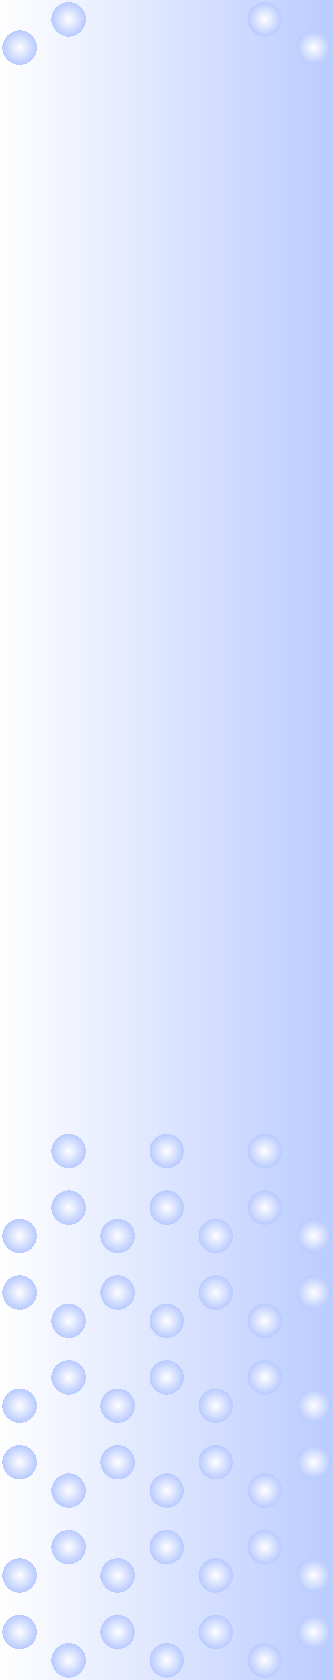
\includegraphics[width=2cm]{Abbildungen/sidebar.pdf}}
\makeatother

\setbeamertemplate{frametitle}{\begin{center} \bfseries \insertframetitle \end{center}}
\setbeamertemplate{itemize item}{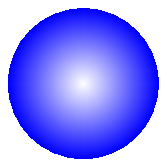
\includegraphics[height=6pt]{Abbildungen/item.pdf}}
\setbeamertemplate{itemize subitem}{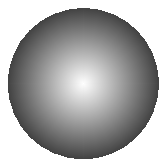
\includegraphics[height=6pt]{Abbildungen/subitem.pdf}}

\newcommand \inlinetitle[1]{\begin{center} \color{MidnightBlue} \bf \Large #1 \end{center}}

\usepackage[utf8]{inputenc}
\usepackage[ngerman]{babel}
\usepackage{amsfonts, amsmath, amssymb, slantsc, mathtools, nicefrac, graphicx}

\usepackage{lmodern}
\usepackage[math]{iwona}
\usepackage{inconsolata}
\usepackage[T1]{fontenc}

\usepackage[skip=0pt, belowskip=0pt]{caption}

\usepackage{color}
\definecolor{grey}{rgb}{0.5, 0.5, 0.5}

\pdfsuppresswarningpagegroup=1

\newcommand \bra[1]{\left \langle #1 \right |}
\newcommand \ket[1]{\left | #1 \right \rangle}
\newcommand \bracket[2]{\left \langle #1 \middle | #2 \right \rangle}

\newcommand \parens[1]{\left ( #1 \right )}
\newcommand \bracks[1]{\left [ #1 \right ]}
\newcommand \braces[1]{\left \lbrace #1 \right \rbrace}

\newcommand \av[1]{\left \langle #1 \right \rangle}
\newcommand \norm[1]{\left \| #1 \right \|}
\newcommand \abs[1]{\left | #1 \right |}
\newcommand \floor[1]{\left \lfloor #1 \right \rfloor}
\newcommand \ceil[1]{\left \lceil #1 \right \rceil}

\def \I {\mathrm i}
\def \E {\mathrm e}
\def \D {\mathrm d}

\def \mod {\bmod}

\def \phi {\varphi}
\def \epsilon {\varepsilon}
\def \vec {\boldsymbol}

\newcommand \op[1]{\mathrm{#1}}
\newcommand \mat[1]{\begin{pmatrix} #1 \end{pmatrix}}
\newcommand \diff[2]{\frac{\D #1}{\D #2}}
\newcommand \pdiff[2]{\frac{\partial #1}{\partial #2}}

\def \eC {\varepsilon_\mathrm{C}}
\def \eX {\varepsilon_\mathrm{X}}
\def \nC {n_\mathrm{C}}
\def \nX {n_\mathrm{X}}
\def \nE {n_\mathrm{e}}
\def \cE {c_\mathrm{e}}
\def \cX {c_\mathrm{X}}

\newcommand \src[6][!]{\bibitem[\textsc{#2}]{#3} \textsc{#4}\ifx!#1\else\ #1\fi: \emph{#5}. #6}

\title{Phasen ladungsabhängiger \\ Adsorbatstrukturen auf Graphen}

\subtitle{Kolloquium zur Bachelorarbeit}

\author[Jan Berges]{
	\scriptsize Jan Berges \\[1pc]
	\hspace{0cm}\llap{Erstgutachter}\hspace{7pt}\rlap{Prof. Dr. Tim Wehling} \\
	\hspace{0cm}\llap{Zweitgutachter}\hspace{7pt}\rlap{Dr. Bálint Aradi}}

\institute{
	Institut für Theoretische Physik \\
	\it Electronic Structure and Correlated Nanosystems}

\date{\tiny 25. September 2014}

\titlegraphic{
\includegraphics[width=3cm]{Abbildungen/Uni.pdf} \hfill 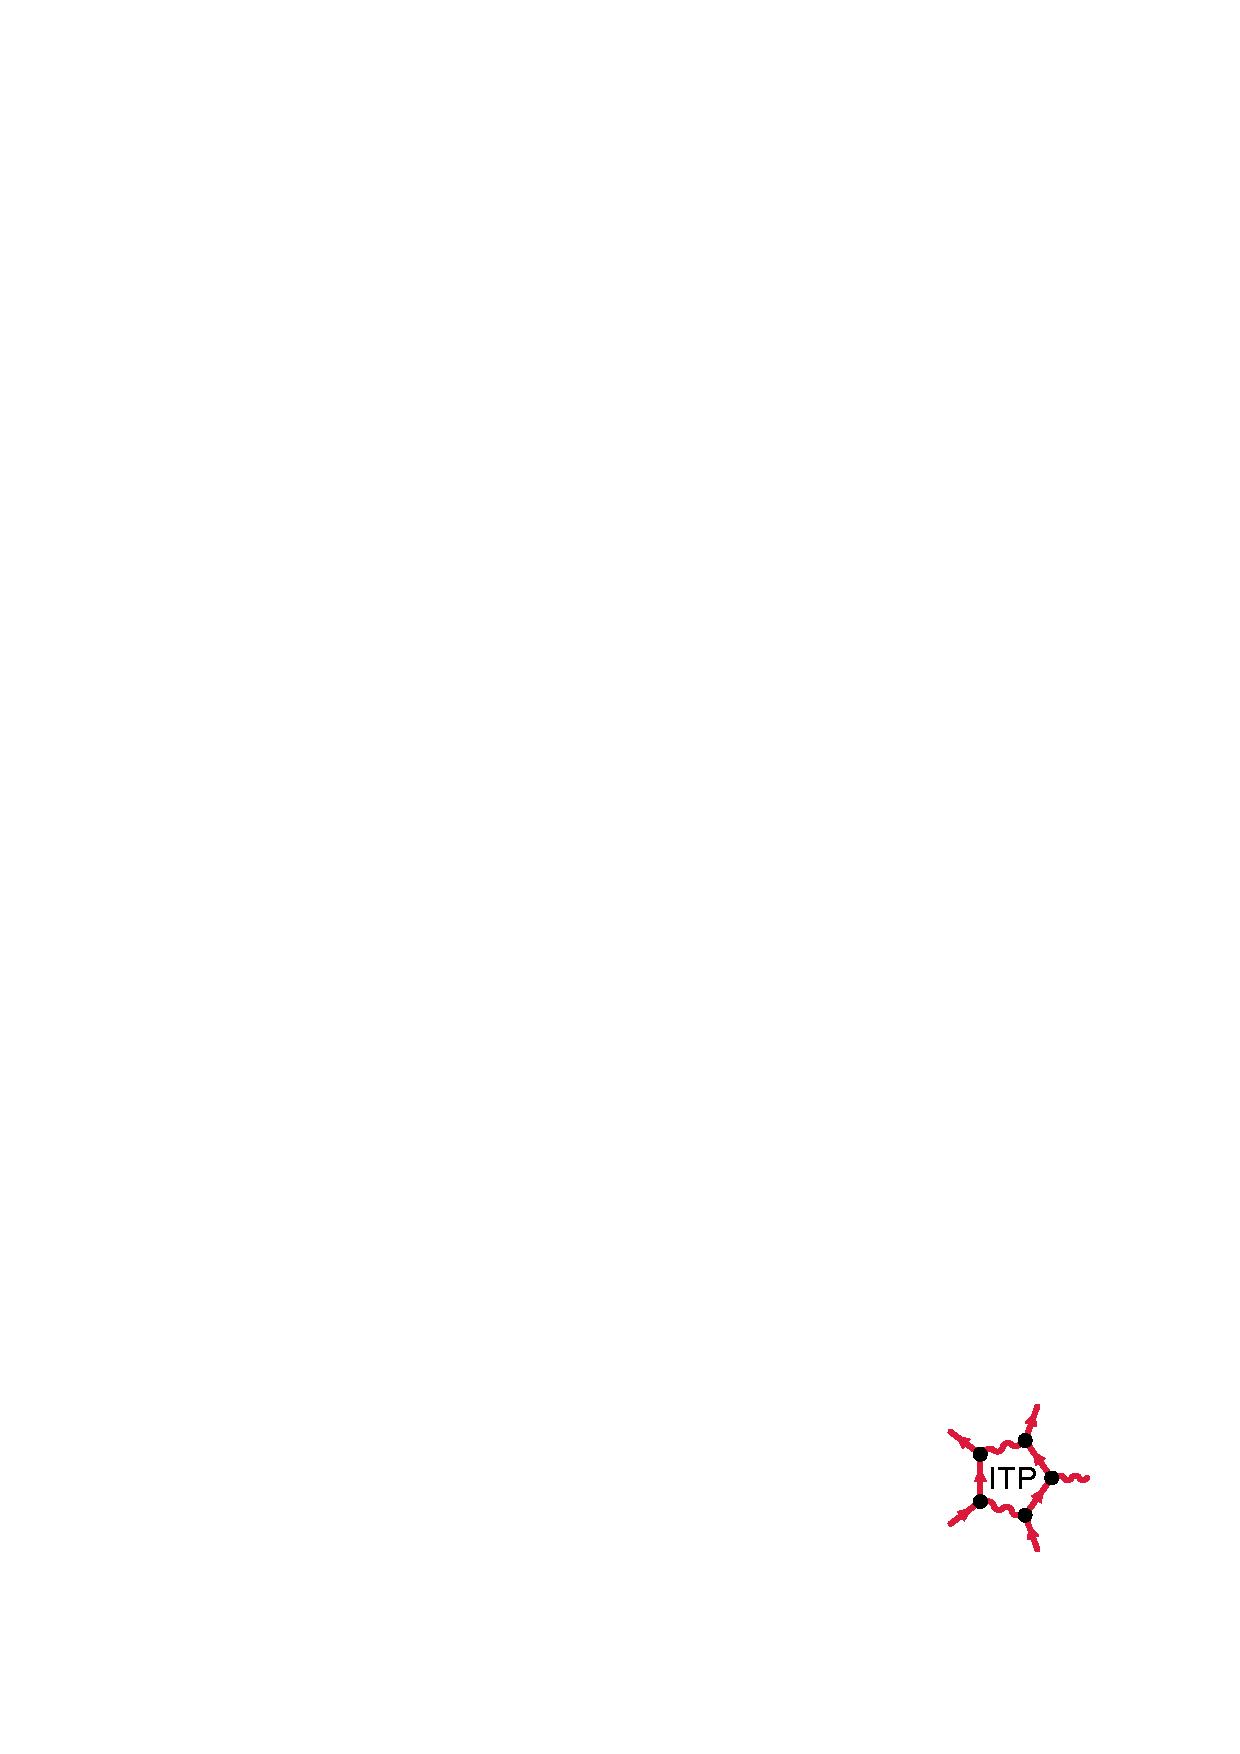
\includegraphics[height=1.5cm]{Abbildungen/ITP.pdf}}

\begin{document}
	\begin{frame}
		\titlepage
	\end{frame}

	\section*{Gliederung}

	\begin{frame}{Gliederung}
		\begin{minipage}{0.35\textwidth}
			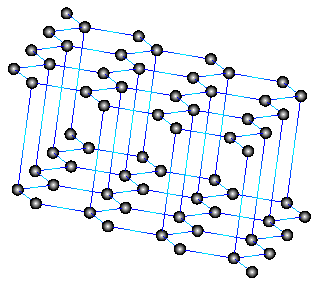
\includegraphics[width=\textwidth, angle=90]{Abbildungen/Raumstrukturen/Graphit.pdf}
		\end{minipage}
		\hfill
		\begin{minipage}{0.60\textwidth}
			\tableofcontents
		\end{minipage}
	\end{frame}

	\section{Motivation}

	\begin{frame}{Motivation}
		\begin{itemize}
			\item viel Spielraum bzgl. chemischer Funktionalisierung
			\begin{itemize}
				\item Isolator $\leftrightarrow$ Halbleiter $\leftrightarrow$ Metall $\leftrightarrow$ Supraleiter
			\end{itemize}
			\item für gegebene $\cE$ und $\cX$ spezielle Konfiguationen der Adsorbate energetisch günstiger als andere\footnote{Ausgangspunkt sind die Ergebnisse von \cite{Wehling}.}
			\item Phasendiagramme bzgl. H- und F-Adsorbaten?
			\begin{itemize}
				\item einfaches Tight-Binding-Modell
				\item Optimierungsverfahren
			\end{itemize}
			\item Ein-/Ausgabe über Programm mit Benutzeroberfläche
		\end{itemize}
		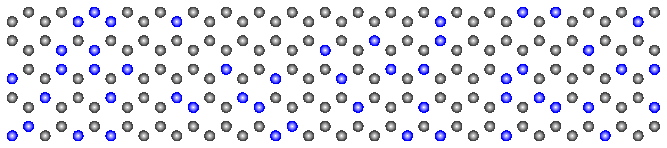
\includegraphics[width=\textwidth]{Abbildungen/motivation.pdf}
	\end{frame}

	\section{Theorie}
	
	\subsection{Festkörperphysik}
	
	\begin{frame}
		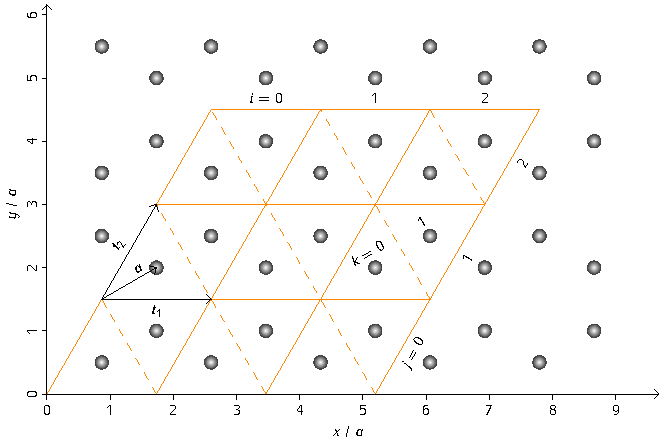
\includegraphics[width=\textwidth]{Abbildungen/Raumstrukturen/Orientierung.pdf}
		%
		\begin{itemize}
			\item Superzelle mit $l \times l$ Elementarzellen
			\item \textsc{Bravais}-Gitter $\vec R = i \vec t_1 + j \vec t_2$ mit $i, j \in \braces{0 \dots l - 1}$
			\item Kohlenstoffatome bei $\vec R + (k + 1) \vec a$ mit $k \in \braces{0, 1}$
		\end{itemize}
	\end{frame}

	\begin{frame}{Das Tight-Binding-Modell}
		\begin{itemize}
			\item \textsc{Wannier}-Zustände $\ket{\vec R}$
			\begin{itemize}
				\item orthonormal und lokalisiert
				\item bei mehratomiger Basis $\ket{\vec R} \ket a, \ket{\vec R} \ket b \dots$
			\end{itemize}
			%
			\item \emph{on-site}-Energie $\epsilon_\mathrm{C} = \bra{\vec R} \op H \ket{\vec R} = 0$
			%
			\item \textit{hopping}-Kopplung $t = 2.6\,\mathrm{eV}$ unmittelbarer Nachbarn
			%
			\begin{align*}
				\bra{\vec R} \op H_t \ket{\vec R\smash'} =
				\begin{cases}
					-t & \text{für } \abs{\vec R - \vec R'} = a \\ 0 & \text{sonst}
				\end{cases}
			\end{align*}
			%
			\item analog für Adsorbate:
			\begin{itemize}
				\item Unterscheidung durch $\eX = \begin{cases} 0 & \text{für Wasserstoff} \\ -2\,\mathrm{eV} & \text{für Fluor} \end{cases}$
				\item Kopplung $V = 6\,\mathrm{eV}$ von Paar aus Fremd- und C-Atom
			\end{itemize}
			\item effektives Einteilchenproblem
		\end{itemize}
	\end{frame}

	\begin{frame}{\textsc{Bloch}-Zustände}
		\begin{itemize}
			\item unitärer Translationsoperator $\op U_{\vec R}$
			%
			\begin{align*}
				\op U_{\vec R'} \ket{\vec R} = \ket{\vec R - \vec R\smash'}
			\end{align*}
			%
			\item \textsc{Hamilton}-Operator $\op H$ und $\op U_{\vec R}$ kommutieren.
			%
			\begin{itemize}
				\item gemeinsames vollständiges Orthonormalsystem
			\end{itemize}
			%
			\item \textsc{Bloch}-Zustände sind Eigenzustände.
			%
			\begin{align*}
				\op U_{\vec R} \ket{\vec k} = \E^{\I \vec R \cdot \vec k} \ket{\vec k}
			\end{align*}
			%
			\item als \textsc{Fourier}-Reihen darstellbar
			\begin{itemize}
				\item nicht normiert, d.h. $\bracket{\vec k}{\vec k\smash'} = B \sum_{\vec K} \delta(\vec k' - \vec k - \vec K)$
				\item \textsc{Wannier}-Zustände als Koeffizienten
			\end{itemize}
			%
			\begin{align*}
				\ket{\vec k} = \sum_{\vec R} \ket{\vec R} \, \E^{\I \vec R \cdot \vec k} \quad \text{mit} \quad \ket{\vec R} = \frac 1 B \int \limits_{\rm BZ} \ket{\vec k} \, \E^{-\I \vec R \cdot \vec k} \, \D^2 k
			\end{align*}
		\end{itemize}
	\end{frame}
	
	\begin{frame}{Bandstruktur reinen Graphens}
		\begin{itemize}
			\item nur $\pi$-Bindungen ($\mathrm p_z$-Orbitale) betrachtet
			%
			\begin{align*}
				H = \eC - t \sum_{\vec R} \bracks{1 + \op U_{\vec t_1} + \op U_{\vec t_2}} \ket{\vec R} \ket a \bra b \bra{\vec R} + \text{h.c.}
			\end{align*}
			%
			\item Entwicklung nach \textsc{Bloch}-Zuständen
			%
			\begin{align*}
				\vec H = \mat{\eC & z \\ \overline z & \eC} \quad \text{mit} \quad z = -t \bracks{1 + \E^{\I \vec t_1 \cdot \vec k} + \E^{\I \vec t_2 \cdot \vec k}}
			\end{align*}
			%
			\item schiefwinklige Koordinaten
			\begin{itemize}
				\item in Einheiten der reziproken Basisvektoren $\vec u_{1, 2}$ mal $2 \pi$
			\end{itemize}
			%
			\begin{align*}
				\quad k_n = \vec t_n \cdot \vec k = \vec t_n \cdot (c_1 \vec u_1 + c_2 \vec u_2) = 2 \pi c_n
			\end{align*}
			%
			\item Lösung über $\det(\vec H - E \vec 1) = 0$
			%
			\begin{align*}
				E_\pm = \eC \mp t \sqrt{3 + 2 \cos(k_1) + 2 \cos(k_2) + 2 \cos(k_2 - k_1)}
			\end{align*}
		\end{itemize}
	\end{frame}
	
	\begin{frame}{Beispiel: Berechnung im Ortsraum}
		\begin{itemize}
			\item Superzelle der Größe $l = 2$
			\item eindeutiger Index $N = \begin{cases} 2 (i l + j) + k & \text{für C-Atome} \\ \nC + n & \text{für Adsorbate} \end{cases}$
		\end{itemize}
		%
		\begin{minipage}[b][0.464\textwidth][c]{0.4\textwidth}
			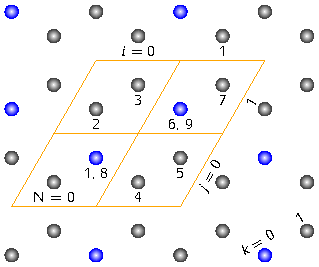
\includegraphics[width=\textwidth]{Abbildungen/Raumstrukturen/Ortsraumbeispiel.pdf}
		\end{minipage}
		\hfill
		\begin{minipage}[b][0.464\textwidth][c]{0.55\textwidth}
			\only<1>{
				\tiny \vspace{-1pc}
				\begin{align*}
					\bordermatrix{
					    \color{grey} N & \color{grey}  0   & \color{grey}  1   & \color{grey}  2   & \color{grey}  3   & \color{grey}  4   & \color{grey}  5   & \color{grey}  6   & \color{grey}  7   & \color{grey} 8   & \color{grey} 9 \cr
						\color{grey} 0 &               \eC & \color{blue} -t   &               0   & \color{red}  -t   &               0   & \color{red}  -t   &               0   &               0   &              0   &              0 \cr
						\color{grey} 1 & \color{blue} -t   &               \eC & \color{blue} -t   &               0   & \color{blue} -t   &               0   &               0   &               0   &              V   &              0 \cr
						\color{grey} 2 &               0   & \color{blue} -t   &               \eC & \color{blue} -t   &               0   &               0   &               0   & \color{red}  -t   &              0   &              0 \cr
						\color{grey} 3 & \color{red}  -t   &               0   & \color{blue} -t   &               \eC &               0   &               0   & \color{blue} -t   &               0   &              0   &              0 \cr
						\color{grey} 4 &               0   & \color{blue} -t   &               0   &               0   &               \eC & \color{blue} -t   &               0   & \color{red}  -t   &              0   &              0 \cr
						\color{grey} 5 & \color{red}  -t   &               0   &               0   &               0   & \color{blue} -t   &               \eC & \color{blue} -t   &               0   &              0   &              0 \cr
						\color{grey} 6 &               0   &               0   &               0   & \color{blue} -t   &               0   & \color{blue} -t   &               \eC & \color{blue} -t   &              0   &              V \cr
						\color{grey} 7 &               0   &               0   & \color{red}  -t   &               0   & \color{red}  -t   &               0   & \color{blue} -t   &               \eC &              0   &              0 \cr
						\color{grey} 8 &               0   &               V   &               0   &               0   &               0   &               0   &               0   &               0   &              \eX &              0 \cr
						\color{grey} 9 &               0   &               0   &               0   &               0   &               0   &               0   &               V   &               0   &              0   &              \eX }
				\end{align*}
				}
			\only<2>{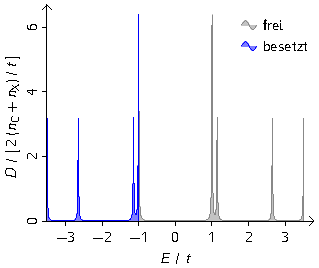
\includegraphics[width=\textwidth]{Abbildungen/Ortsraumbeispiel.pdf}}
		\end{minipage}
		%
		\begin{minipage}[t][2cm][t]{\textwidth}
			\vspace*{-4mm}
			\begin{itemize}
				\only<1>{
					\item[\color{blue} $-t$] \emph{hopping} innerhalb einer Superzelle\dots
					\item[\color{red}  $-t$] \dots und über deren Grenzen hinweg
					}
				\only<2>{
					\item acht unterschiedliche Energieeigenwerte
					\begin{itemize}
						\item davon zwei mit zweifacher Entartung
					\end{itemize}
					\item Gesamtenergie ist Summe der kleinsten $\nE$ Energien
					}
			\end{itemize}
		\end{minipage}
	\end{frame}
	
	\subsection{Optimierung}

	\begin{frame}{Der Hill-Climbing-Algorithmus}
		Ausgehend von Ausgangszustand der Energie $E_0$:
		\begin{enumerate}
			\item Variiere Konfiguration.
			\begin{itemize}
				\item gleichverteilte Zufallszahlen
				%
				\begin{align*}
					r \in [0, R] \quad \text{und} \quad \phi \in [0, 2 \pi]
				\end{align*}
				%
				\item Weise einem Fremdatom bei $(x_0 \ y_0)$ neuen Ort mit
				%
				\begin{align*}
					x = x_0 + r \cos(\phi) \quad \text{und} \quad y = y_0 + r \sin(\phi)
				\end{align*}
				%
				zu, der auf eine Kohlenstoffposition gerundet wird.
			\end{itemize}
			\item Ist der Platz frei und die neue Energie $E < E_0$?
			\begin{itemize}
				\item[\emph{Ja:}] Akzeptiere Schritt und setzte $E_0 = E$.
				\item[\emph{Nein:}] Bleibe beim alten Zustand.
			\end{itemize}
			\item[$\circlearrowleft$] Wiederhole für nächstes Fremdatom.
		\end{enumerate}
		So ist jedes erreichte lokale Minimum endgültig.
	\end{frame}
	
	\begin{frame}{Zustandsdichten kleiner Systeme}
		\begin{itemize}
			\item Ensembles kleiner Systeme vollständig betrachtbar
			\begin{itemize}
				\item $\nC! \, / \, \bracks{\nX! \ (\nC - \nX)!}$ teils äquivalente Konfigurationen
			\end{itemize}
		\end{itemize}
		\begin{figure}
			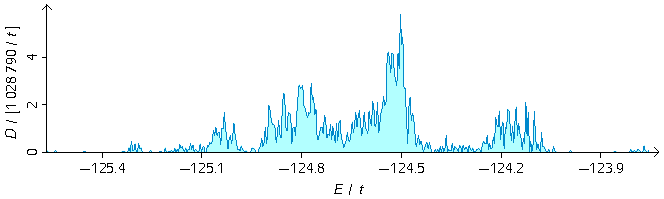
\includegraphics[width=\textwidth]{Abbildungen/75.pdf} \\
			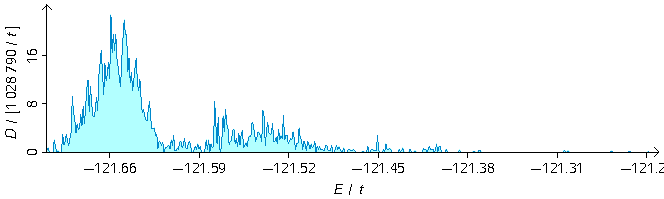
\includegraphics[width=\textwidth]{Abbildungen/84.pdf}
			\caption{Für $\nC = 72$, $\nX = 4$ und $\cE = 0$ (oben) bzw. $0.125$ (unten)}
		\end{figure}
	\end{frame}
	
	\section{Auswertung}
	
	\subsection{Beschreibende Größen}

	\begin{frame}{Gruppiertheit}
		\begin{itemize}
			\item[${\nX}_i$] Größe der $i$-ten Fremdatomgruppe, die durch direkte Nachbarschaft verbunden ist
			%
			\begin{align*}
				G = \begin{cases} \frac{\sum_i ({\nX}_i - 1) {\nX}_i}{(\nX - 1) \nX} & \nX > 1 \\ 0 & \text{sonst} \end{cases} \quad \text{mit} \quad \nX = \sum_i {\nX}_i
			\end{align*}
			%
			\item Für $\nX > 1$ folgt $G$ aus $\tilde G$ über Streckung dessen Wertebereichs von $[\nX^{-1}, 1]$ auf $[0, 1]$.
			%
			\begin{align*}
				G  = \frac{\nX \tilde G - 1}{\nX - 1} \quad \text{mit} \quad \tilde G = \frac{\sum_i {\nX^2}_i}{\nX^2}
			\end{align*}
			%
			\item von Gruppenform und -größe unabhängig
		\end{itemize}
	\end{frame}

	\begin{frame}{Kompaktheit}
		\begin{itemize}
			\item Maß für die Minimierung des Randbereichs von Fremdatomgruppen
			%
			\begin{align*}
				K = \begin{cases} \frac 2 3 \frac{\text{Anzahl direkter Nachbarschaften}}{\text{Anzahl Fremdatome}} & \nX \neq 0 \\ 0 & \text{sonst} \end{cases}
			\end{align*}
			%
			\item $K \in [0, 1]$
			\item proportional zum Gesamtpenalty
			\begin{itemize}
				\item[] $P = \text{Nachbarschaften} \cdot p = 1.5 \, K \, \nX \, p$
				
				\medskip
				
				\item Kovalente Adsorbatbindung hebt C-Atom aus der Ebene und rehybridisiert lokal von $\rm sp^2$ zu $\rm sp^3$ \cite{Wehling}.
				\item Modellabweichungen bei benachbarten Fremdatomen
				\begin{itemize}
					\item[$\rightarrow$] Kompensation durch \emph{Penalty} $p = 0.5\,\mathrm{eV}$
				\end{itemize}
			\end{itemize}
		\end{itemize}
	\end{frame}

	\begin{frame}{Lokale Distanz}
		\begin{itemize}
			\item mittlerer Abstand eines Fremdatoms zum jeweils nächsten Nachbarn
			\begin{itemize}
				\item Abstand gemessen in Kanten des Wabengitters
			\end{itemize}
			\item Wertebereich $[0, \infty]$ bzw. $[0, 2 l]$ für Superzelle
			\item frei von Oberflächen- bzw. in 2D Randeffekten
			\item Charakterisiert Inseln, innerhalb derer die Fremdatome einen konstanten Abstand aufweisen.
		\end{itemize}
	\end{frame}

	\begin{frame}{(Untergitter-) Polarisierung}
		\begin{itemize}
			\item Durch Bevorzugung eines der beiden Untergitter A oder B wird eine Symmetrie gebrochen.
			\item[$\nX^\text{A/B}$] Anzahl der Fremdatome auf A bzw. B
			%
			\begin{align*}
				P = \begin{cases} \abs{1 - 2 \nX^\text{B} \nX^{-1}} & \nX \neq 0 \\ 0 & \text{sonst} \end{cases} \quad \text{mit} \quad \nX = \nX^\text{A} + \nX^\text{B}
			\end{align*}
			%
			\item $P \in [0, 1]$
			\item Ordnungsparameter
			\begin{itemize}
				\item größerer Wert $\leftrightarrow$ höhere Ordnung
			\end{itemize}
		\end{itemize}
	\end{frame}

	\subsection{Phasen}
	
	\begin{frame}{Aufgetretene Phasen}
		\begin{figure}
			\scriptsize
			\begin{minipage}[b]{0.32\textwidth}
				\centering
				$\rm C_2X_2$
				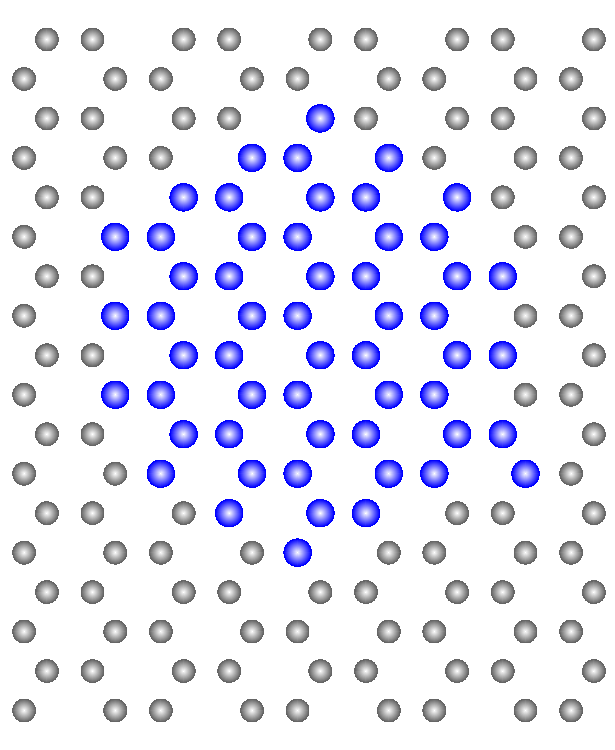
\includegraphics[width=0.85\textwidth, angle=90]{Abbildungen/C2X2.pdf}
			\end{minipage}
			\hfill
			\begin{minipage}[b]{0.32\textwidth}
				\centering
				$\rm C_8X_2$
				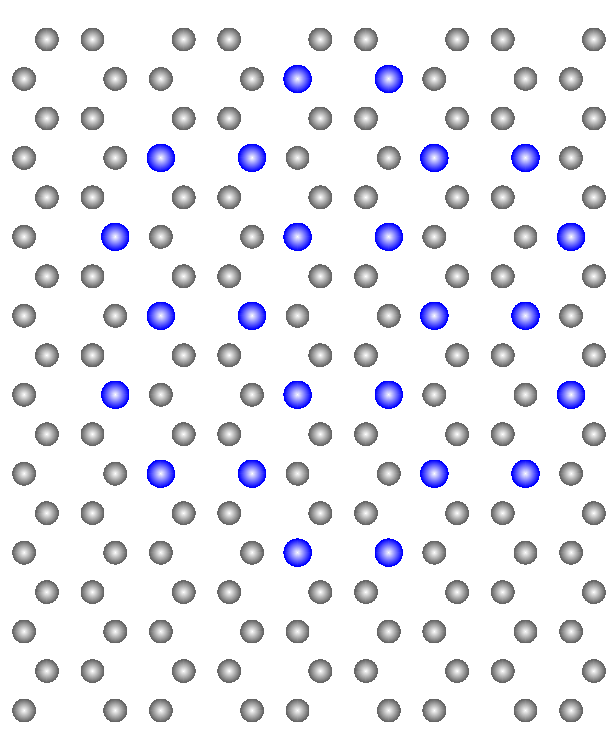
\includegraphics[width=0.85\textwidth, angle=90]{Abbildungen/Raumstrukturen/superzelle.pdf}
			\end{minipage}
			\hfill
			\begin{minipage}[b]{0.32\textwidth}
				\centering
				ungeordnet
				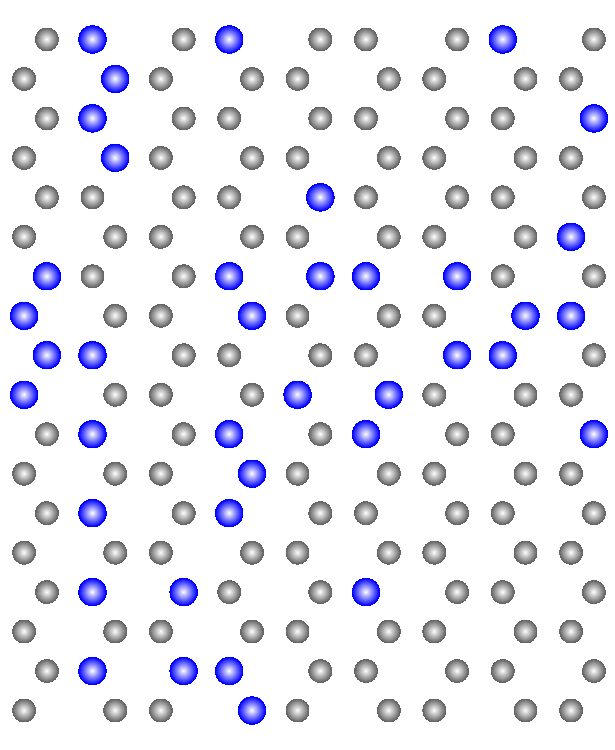
\includegraphics[width=0.85\textwidth, angle=90]{Abbildungen/random.pdf}
			\end{minipage}
			
			\medskip
			
			\begin{minipage}[t]{0.32\textwidth}
				\centering
				$\rm C_2X$
				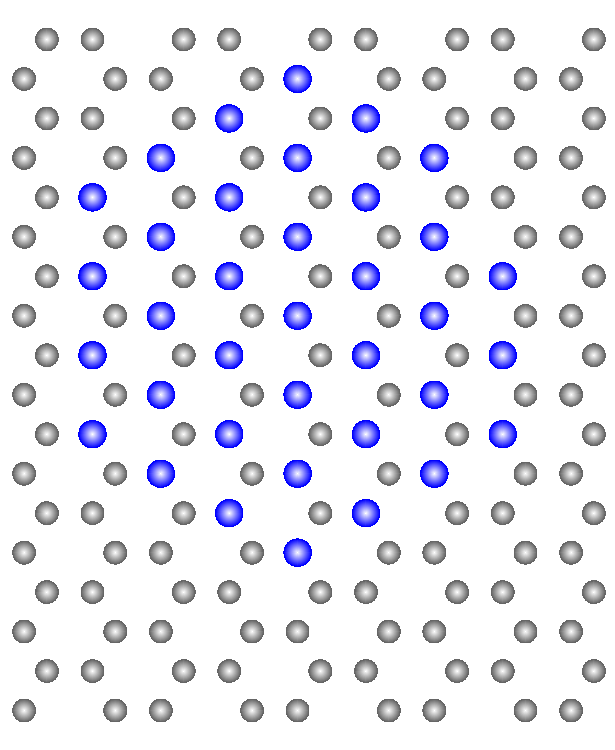
\includegraphics[width=0.85\textwidth, angle=90]{Abbildungen/C2X.pdf}
			\end{minipage}
			\hfill
			\begin{minipage}[t]{0.32\textwidth}
				\centering
				$\rm C_6X$
				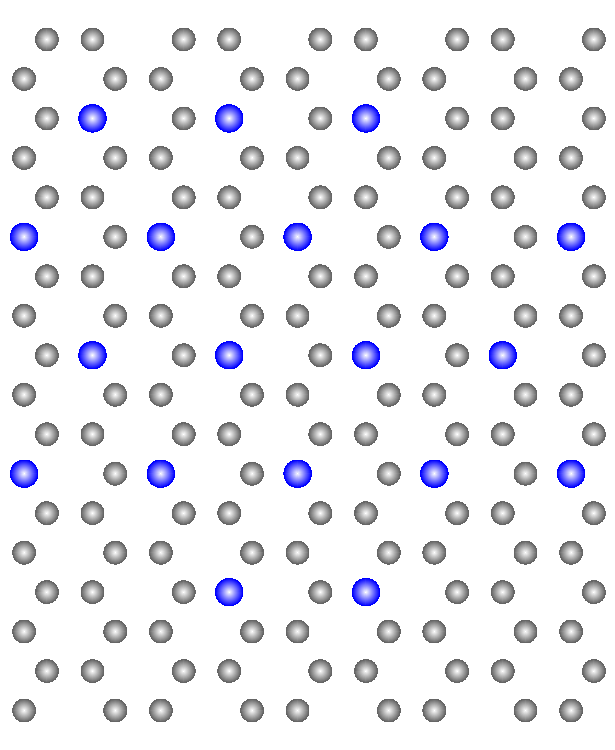
\includegraphics[width=0.85\textwidth, angle=90]{Abbildungen/C6X.pdf}
			\end{minipage}
			\hfill
			\parbox[t]{0.25\textwidth}{
				\caption{Partielle Besetzung durch die fünf Standardkonfigurationen}
				}
		\end{figure}
	\end{frame}
	
	\begin{frame}
		\begin{minipage}[b][0.48\textwidth][c]{0.48\textwidth}
			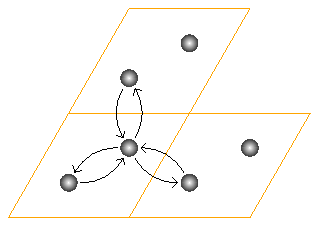
\includegraphics[width=\textwidth]{Abbildungen/Raumstrukturen/Graphen.pdf}
		\end{minipage}
		\hfill
		\begin{minipage}[b][0.48\textwidth][c]{0.48\textwidth}
			\only<1>{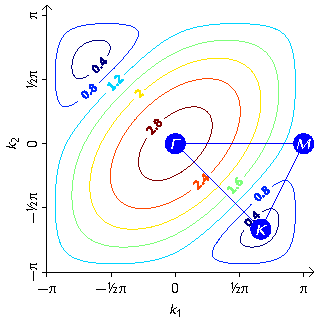
\includegraphics[width=\textwidth]{Abbildungen/Bandstrukturen/BZ_C2_1.pdf}}
			\only<2>{
				\inlinetitle{$\mathbf C_{\boldsymbol 2}$}
				\begin{itemize}
					\item "`Graphen"'
					\item \textsc{Dirac}-Material
					\begin{itemize}
						\item zwischen Metall und Halbleiter
						\item lineare Dispersion auf \textsc{Fermi}-Niveau
					\end{itemize}
				\end{itemize}
				}
		\end{minipage}
		%
		\begin{minipage}{0.48\textwidth}
			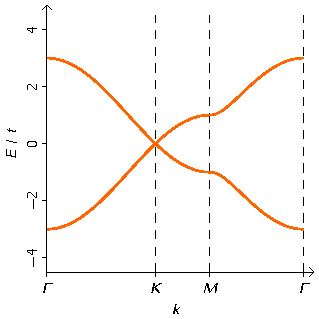
\includegraphics[width=\textwidth]{Abbildungen/Bandstrukturen/C2.pdf}
		\end{minipage}
		\hfill
		\begin{minipage}{0.48\textwidth}
			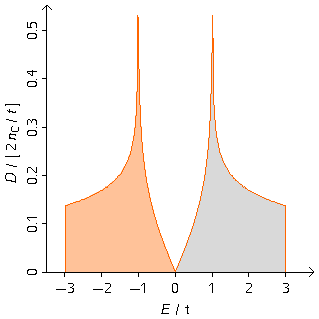
\includegraphics[width=\textwidth]{Abbildungen/Bandstrukturen/DOS_C2_2.pdf}
		\end{minipage}
	\end{frame}
	
	\begin{frame}
		\begin{minipage}[b][0.48\textwidth][c]{0.48\textwidth}
			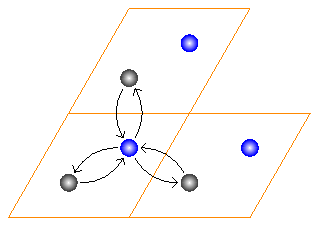
\includegraphics[width=\textwidth]{Abbildungen/Raumstrukturen/C2X.pdf}
		\end{minipage}
		\hfill
		\begin{minipage}[b][0.48\textwidth][c]{0.48\textwidth}
			\inlinetitle{$\bf C_{\boldsymbol 2}X$}
			\begin{itemize}
				\item Peak bei/nahe $E_\text{F}$
				\begin{itemize}
					\item Entartung für Fluor aufgehoben
				\end{itemize}
				\item daneben Bandlücken
				\item $D = 2$, $P = 1$, $G = K = 0$
			\end{itemize}
		\end{minipage}
		%
		\begin{minipage}{0.48\textwidth}
			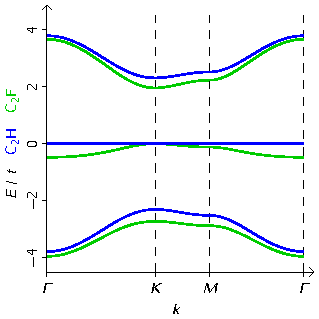
\includegraphics[width=\textwidth]{Abbildungen/Bandstrukturen/C2X.pdf}
		\end{minipage}
		\hfill
		\begin{minipage}{0.48\textwidth}
			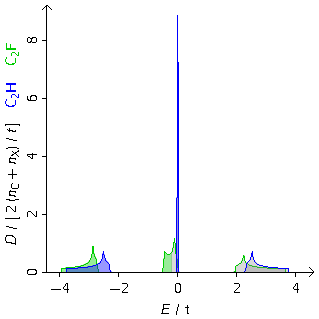
\includegraphics[width=\textwidth]{Abbildungen/Bandstrukturen/DOS_C2X.pdf}
		\end{minipage}
	\end{frame}
	
	\begin{frame}
		\begin{minipage}[b][0.48\textwidth][c]{0.48\textwidth}
			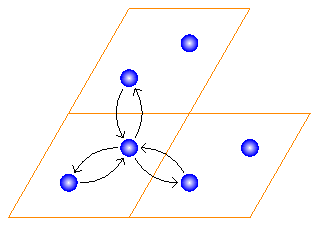
\includegraphics[width=\textwidth]{Abbildungen/Raumstrukturen/C2X2.pdf}
		\end{minipage}
		\hfill
		\begin{minipage}[b][0.48\textwidth][c]{0.48\textwidth}
			\inlinetitle{$\bf C_{\boldsymbol 2}X_{\boldsymbol 2}$}
			\begin{itemize}
				\item "`Graphan"'
				\item Isolator
				\item $D = 1$, $P = 0$, $G = K = 1$
			\end{itemize}
		\end{minipage}
		%
		\begin{minipage}{0.48\textwidth}
			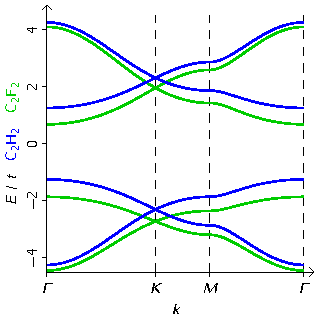
\includegraphics[width=\textwidth]{Abbildungen/Bandstrukturen/C2X2.pdf}
		\end{minipage}
		\hfill
		\begin{minipage}{0.48\textwidth}
			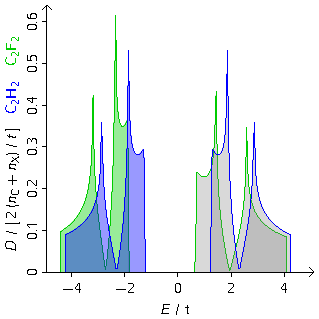
\includegraphics[width=\textwidth]{Abbildungen/Bandstrukturen/DOS_C2X2.pdf}
		\end{minipage}
	\end{frame}
	
	\begin{frame}
		\begin{minipage}[b][0.48\textwidth][c]{0.48\textwidth}
			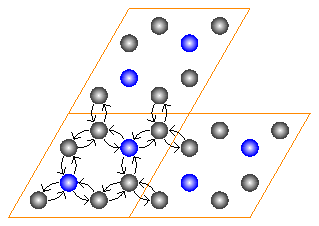
\includegraphics[width=\textwidth]{Abbildungen/Raumstrukturen/C8X2.pdf}
		\end{minipage}
		\hfill
		\begin{minipage}[b][0.48\textwidth][c]{0.48\textwidth}
			\inlinetitle{$\bf C_{\boldsymbol 8}X_{\boldsymbol 2}$}
			\begin{itemize}
				\item Bandlücke bei $E_\text{F}$
				\item $D = 3$, $P = 0$, $G = K = 0$
			\end{itemize}
		\end{minipage}
		%
		\begin{minipage}{0.48\textwidth}
			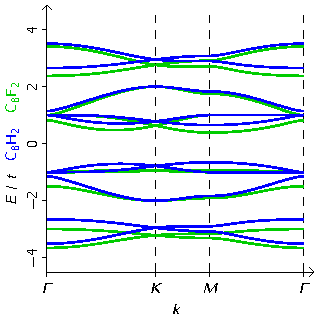
\includegraphics[width=\textwidth]{Abbildungen/Bandstrukturen/C8X2.pdf}
		\end{minipage}
		\hfill
		\begin{minipage}{0.48\textwidth}
			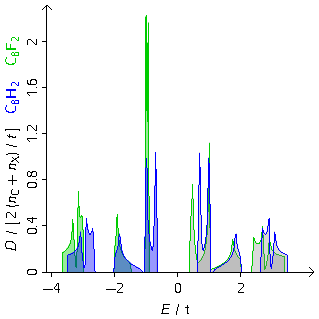
\includegraphics[width=\textwidth]{Abbildungen/Bandstrukturen/DOS_C8X2.pdf}
		\end{minipage}
	\end{frame}
	
	\begin{frame}
		\begin{minipage}[b][0.48\textwidth][c]{0.48\textwidth}
			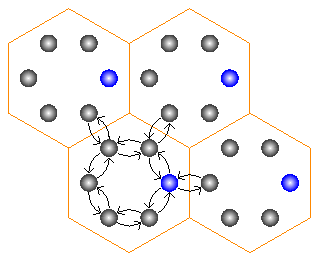
\includegraphics[width=\textwidth]{Abbildungen/Raumstrukturen/Sechstel.pdf}
		\end{minipage}
		\hfill
		\begin{minipage}[b][0.48\textwidth][c]{0.48\textwidth}
			\inlinetitle{$\bf C_{\boldsymbol 6}X$}
			\begin{itemize}
				\item Peak bei/nahe $E_\text{F}$
				\item $D = 4$, $P = 1$, $G = K = 0$
			\end{itemize}
		\end{minipage}
		%
		\begin{minipage}{0.48\textwidth}
			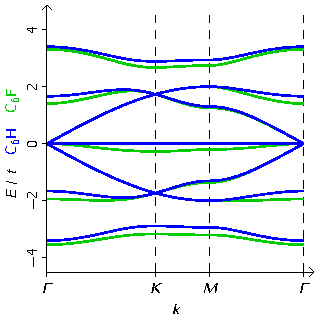
\includegraphics[width=\textwidth]{Abbildungen/Bandstrukturen/C6X.pdf}
		\end{minipage}
		\hfill
		\begin{minipage}{0.48\textwidth}
			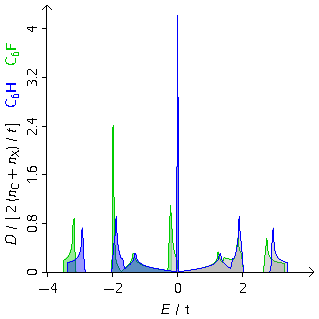
\includegraphics[width=\textwidth]{Abbildungen/Bandstrukturen/DOS_C6X.pdf}
		\end{minipage}
	\end{frame}
	
	\begin{frame}
		\begin{figure}
			\scriptsize
			\begin{minipage}[b]{0.4\textwidth}
				\centering
				$p = 0$
				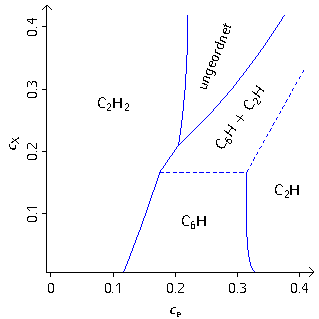
\includegraphics[width=\textwidth]{Abbildungen/Phasendiagramme/Schemata/H.pdf}
			\end{minipage}
			\begin{minipage}[b]{0.4\textwidth}
				\centering
				$p = 0.5\,\mathrm{eV}$
				\only<1>{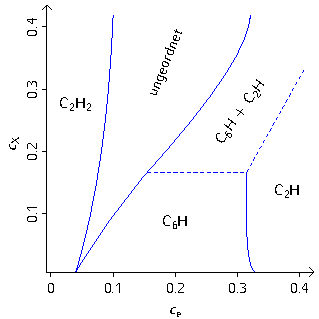
\includegraphics[width=\textwidth]{Abbildungen/Phasendiagramme/Schemata/H_penalty.pdf}}
				\only<2>{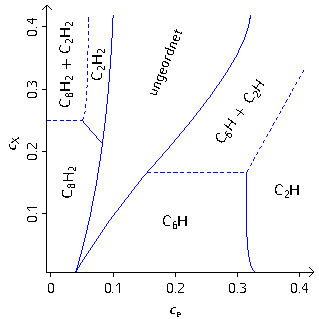
\includegraphics[width=\textwidth]{Abbildungen/Phasendiagramme/Schemata/H_penalty_2.pdf}}
			\end{minipage}
			\begin{minipage}[b]{0.4\textwidth}
				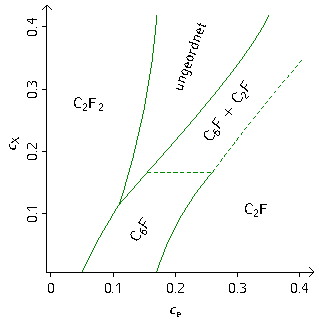
\includegraphics[width=\textwidth]{Abbildungen/Phasendiagramme/Schemata/F.pdf}
			\end{minipage}
			\begin{minipage}[b]{0.4\textwidth}
				\only<1>{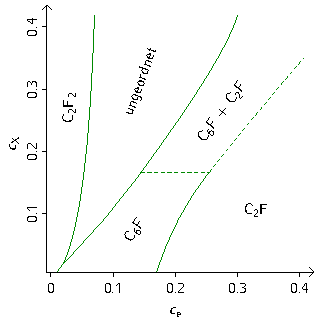
\includegraphics[width=\textwidth]{Abbildungen/Phasendiagramme/Schemata/F_penalty.pdf}}
				\only<2>{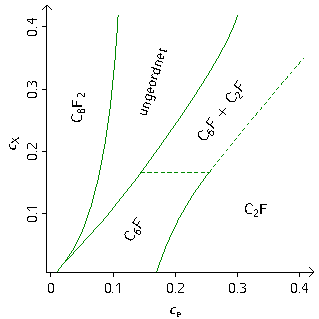
\includegraphics[width=\textwidth]{Abbildungen/Phasendiagramme/Schemata/F_penalty_2.pdf}}
			\end{minipage}
			\caption{Präferenz einer der \only<1>{vier}\only<2>{fünf} Standardkonfigurationen für $l = 18$}
		\end{figure}
	\end{frame}
	
	\begin{frame}{Einfluss der Startkonfiguration}
		\begin{itemize}
			\item Clusterbildung schwieriger als -sprengung
			\begin{itemize}
				\item Variation bewegt nur ein Fremdatom
				\item[$\rightarrow$] gemeinsame Gruppenbewegung unmöglich
			\end{itemize}
			\item Bildung von Domänen und Antiphasengrenzen
			\begin{itemize}
				\item gleiche periodische Struktur, verschiedene Untergitter
				\item[$\rightarrow$] Untergittersymmetrie lokal, aber nicht global \rlap{gebrochen}
			\end{itemize}
		\end{itemize}
		\begin{figure}[b]
			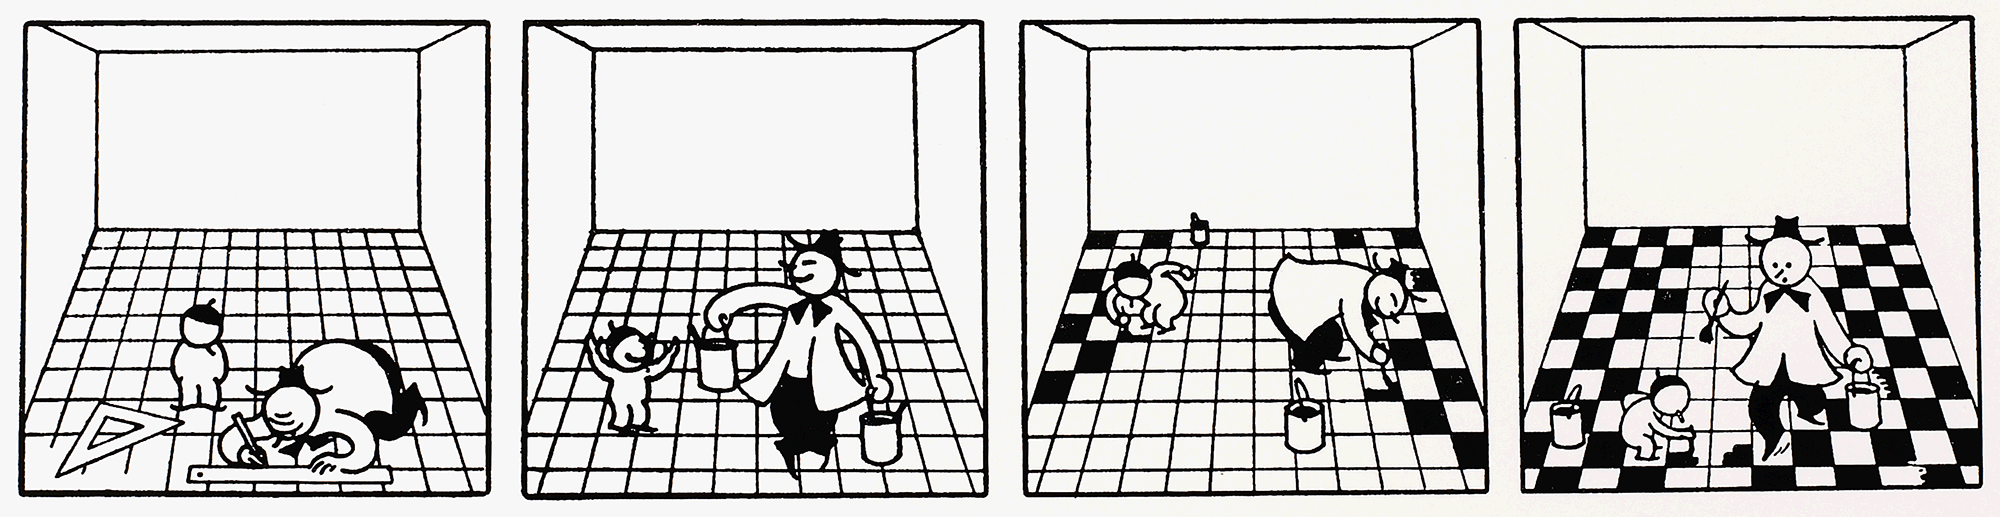
\includegraphics[width=\textwidth]{Abbildungen/hein.png}
			\caption{Antiphasengrenze -- \emph{Painting the floor} von \textsc{Piet Hein}}
		\end{figure}
	\end{frame}

	\subsection{Übergänge}

	\begin{frame}{$\bf C_{\boldsymbol 2}X_{\boldsymbol 2} \rightarrow C_{\boldsymbol 6}X \rightarrow C_{\boldsymbol 2}X$}
		\begin{figure}
			\scriptsize
			\begin{minipage}{0.48\textwidth}
				\centering
				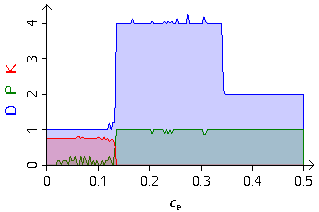
\includegraphics[width=\textwidth]{Abbildungen/C2X2-C6X-C2X.pdf} \\
				$l = 12$, individueller Start
			\end{minipage}
			\hfill
			\begin{minipage}{0.48\textwidth}
				\centering
				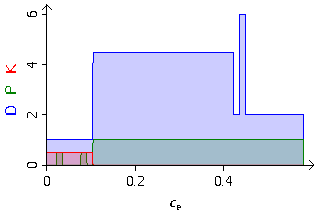
\includegraphics[width=\textwidth]{Abbildungen/C2X2-C6X-C2X-exact.pdf} \\
				$l = 6$, globale Minima
			\end{minipage}
		\end{figure}
		\begin{itemize}
			\item "`Schnitt"' durch Phasendiagramm bei $\cX = \nicefrac 1 {18}$
			\item zwei diskontinuierliche Phasenübergänge
		\end{itemize}
		\begin{figure}
			\scriptsize
			\begin{minipage}[b]{0.19\textwidth}
				\centering
				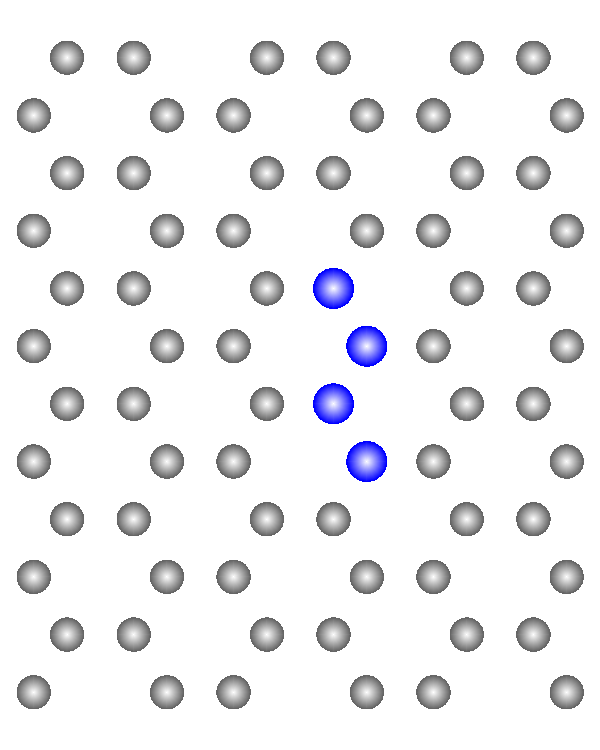
\includegraphics[height=1.1\textwidth]{Abbildungen/ne83.pdf} \\
				$\nE = 83$
			\end{minipage}
			\hfill
			\begin{minipage}[b]{0.19\textwidth}
				\centering
				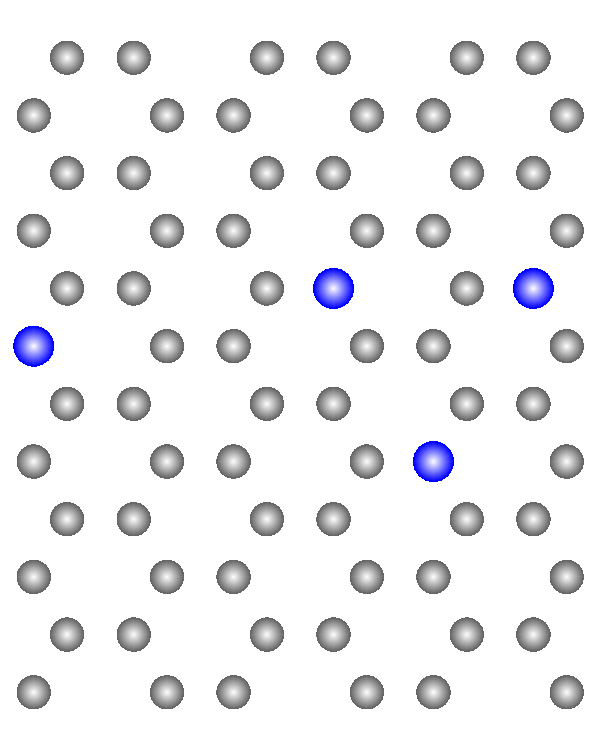
\includegraphics[height=1.1\textwidth]{Abbildungen/ne84.pdf} \\
				$\nE = 84$
			\end{minipage}
			\hfill
			\begin{minipage}[b]{0.19\textwidth}
				\centering
				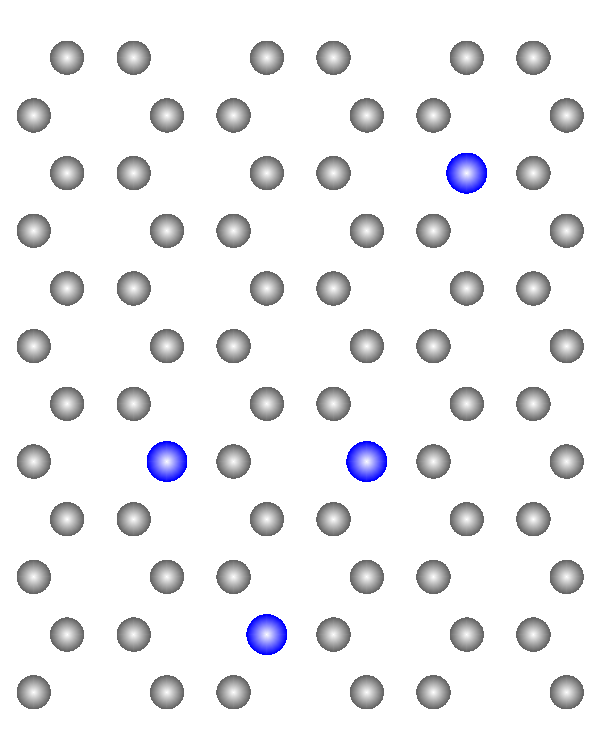
\includegraphics[height=1.1\textwidth]{Abbildungen/ne106.pdf} \\
				$\nE = 106$
			\end{minipage}
			\hfill
			\begin{minipage}[b]{0.19\textwidth}
				\centering
				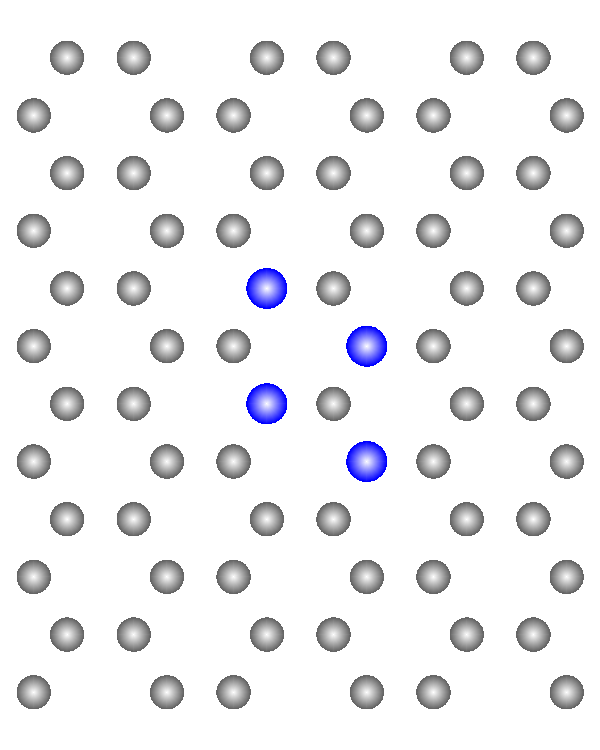
\includegraphics[height=1.1\textwidth]{Abbildungen/ne107.pdf} \\
				$\nE = 107$
			\end{minipage}
			\hfill
			\begin{minipage}[b]{0.19\textwidth}
				\centering
				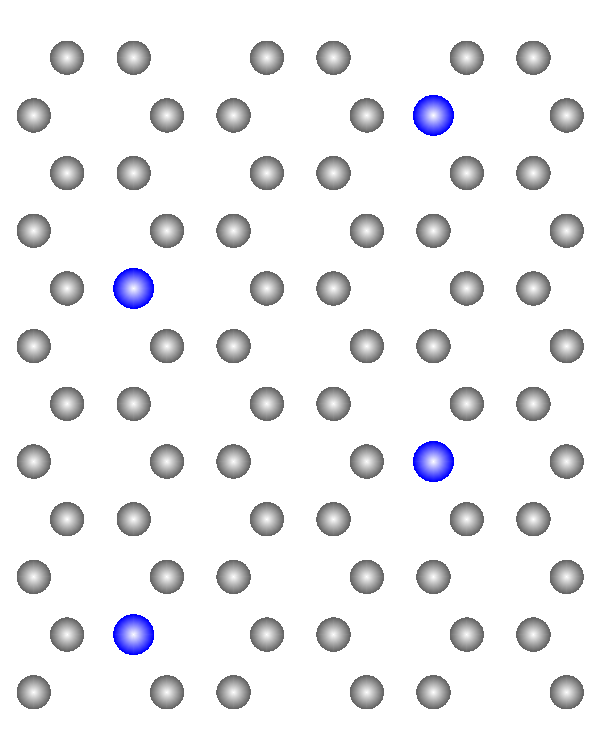
\includegraphics[height=1.1\textwidth]{Abbildungen/ne108.pdf} \\
				$\nE = 108$
			\end{minipage}
		\end{figure}
	\end{frame}
	
	\begin{frame}{$\bf C_{\boldsymbol 2}X_{\boldsymbol 2} \rightarrow$ ungeordnet}
		\begin{figure}
			\scriptsize
			\begin{minipage}{0.48\textwidth}
				\centering
				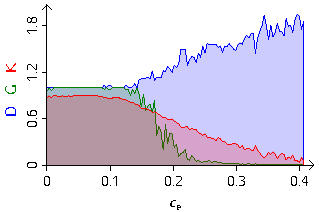
\includegraphics[width=\textwidth]{Abbildungen/C2X2-random.pdf} \\
				$l = 12$, Clustersprengung
			\end{minipage}
			\hfill
			\begin{minipage}{0.48\textwidth}
				\centering
				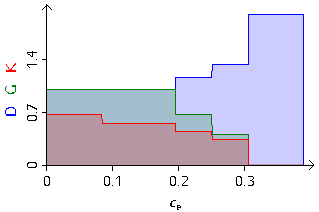
\includegraphics[width=\textwidth]{Abbildungen/C2X2-random-exact.pdf} \\
				$l = 3$, globale Minima
			\end{minipage}
		\end{figure}
		\begin{itemize}
			\item "`Schnitt"' durch Phasendiagramm bei $\cX = \nicefrac 1 3$
			\item kontinuierlicher Verlauf, insbesondere für $K$
		\end{itemize}
		\begin{figure}
			\scriptsize
			\begin{minipage}[b]{0.19\textwidth}
				\centering
				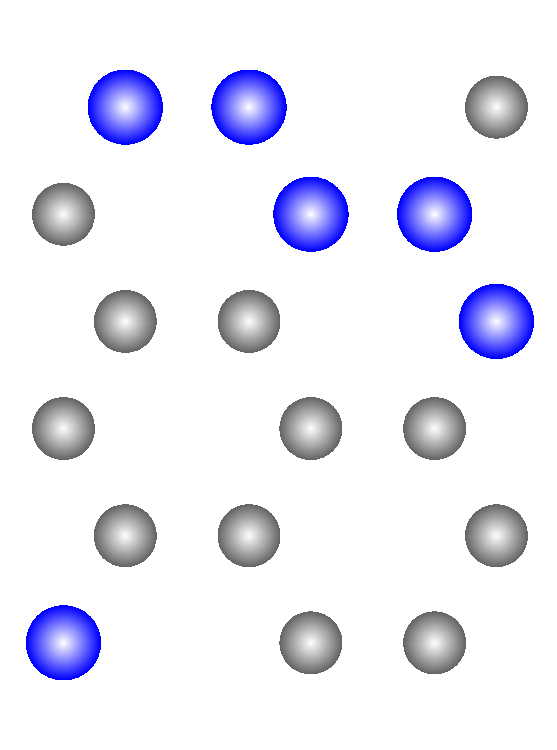
\includegraphics[height=1.1\textwidth]{Abbildungen/1.pdf} \\
				$\nE = 24$
			\end{minipage}
			\hfill
			\begin{minipage}[b]{0.19\textwidth}
				\centering
				\includegraphics[height=1.1\textwidth]{Abbildungen/2.pdf} \\
				$\nE = 26$
			\end{minipage}
			\hfill
			\begin{minipage}[b]{0.19\textwidth}
				\centering
				\includegraphics[height=1.1\textwidth]{Abbildungen/3.pdf} \\
				$\nE = 28$
			\end{minipage}
			\hfill
			\begin{minipage}[b]{0.19\textwidth}
				\centering
				\includegraphics[height=1.1\textwidth]{Abbildungen/4.pdf} \\
				$\nE = 29$
			\end{minipage}
			\hfill
			\begin{minipage}[b]{0.19\textwidth}
				\centering
				\includegraphics[height=1.1\textwidth]{Abbildungen/5.pdf} \\
				$\nE = 30$
			\end{minipage}
		\end{figure}
	\end{frame}

	\section{Zusammenfassung}

	\begin{frame}
		\inlinetitle{Zusammenfassung}
		\begin{itemize}
			\item Verwendung von exaktem und Optimierungsverfahren
			\item Identifizierung von vier bzw. fünf verschiedenen Phasen
			\item Definition beschreibender Größen
			\item kontinuierliche sowie sprunghafte Übergänge
		\end{itemize}
		\medskip
		\inlinetitle{Ausblick}
		\begin{itemize}
			\item anderweitige Verifizierung der Ergebnisse
			\item Erweiterung der verwendeten Modells
			\item Bedeutung für elektronische Struktur?
			\item weitere Materialeigenschaften?
		\end{itemize}
	\end{frame}

	\section{Referenzen}

	\begin{frame}%[allowframebreaks]
		\frametitle{Referenzen}
		
		\begin{thebibliography}{\hspace{1cm}}
			\src{Czy}{Czycholl}{G. Czycholl}{Theoretische Festkörperphysik. Von den klassischen Modellen zu modernen Forschungsthemen}{Springer-Verlag, Berlin/Heidelberg, 2008
			
			\medskip
			
			{\small $\rightarrow$ für die Grundlagen der Festkörperphysik}}
			
			\medskip
			
			\src[et al.]{Weh}{Wehling}{T. O. Wehling}{Charge doping induced phase transitions in hydrogenated and fluorinated graphene}{Physical Review B, Vol. 90, August 2014
			
			\medskip
			
			{\small $\rightarrow$ Ausgangspunkt dieser Arbeit}}
			
			\medskip
			
			\src{Hei}{Hein}{P. Hein}{Painting the floor}{\url{http://www.piethein.dk/}, 17. September 2014}
		\end{thebibliography}
	\end{frame}
	
	\begin{frame}
		\inlinetitle{Programmdemonstration}
		$\rightarrow$ \url{http://localhost/~jan/adsorbatesongraphene/}
	\end{frame}
\end{document}
